
\section{System Framework}
\label{sec:system_framework}

AgenticMobility connects role-specific decisions and persistent states to a shared execution environment. Figure~\ref{fig:framework} summarizes the interaction loop. The framework defines responsibilities for observations, action validation, execution, and feedback; each study supplies the supported roles and environmental realization.


\begin{figure}[htbp]
    \centering
    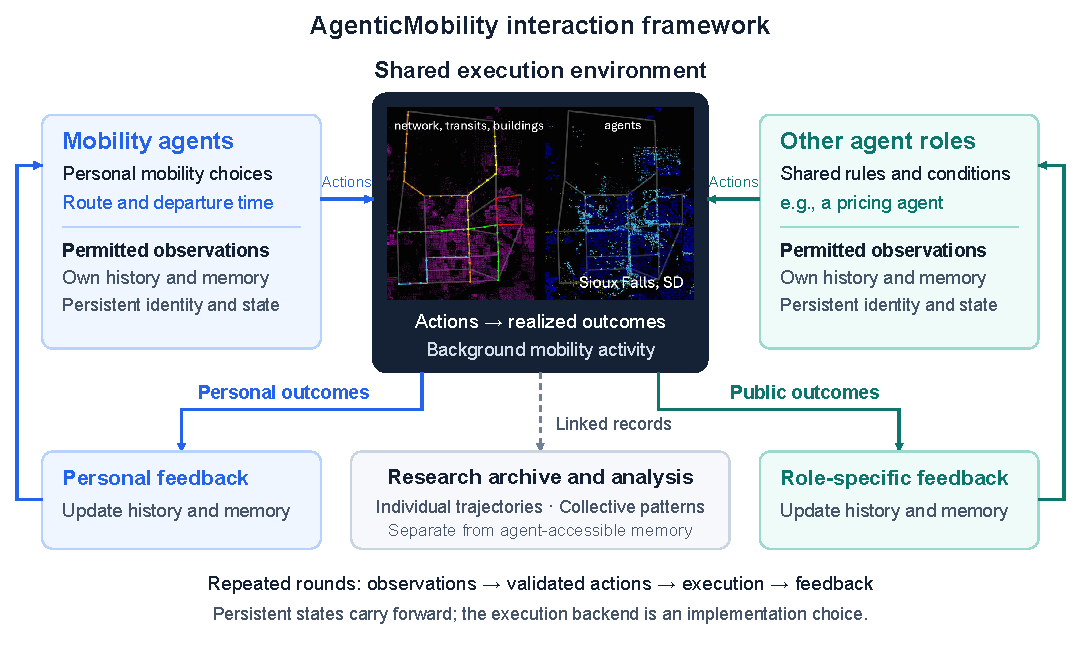
\includegraphics[width=1\textwidth, trim=0cm 1cm 0cm 1cm, clip]{pic/agenticmobility_framework_siouxfalls.pdf}
    \caption{AgenticMobility interaction framework.
Agents submit actions to a shared execution environment
and receive feedback according to their roles.
Persistent states carry experience across rounds, while
a separate research archive links decisions, execution,
and outcomes for analysis.}
    \label{fig:framework}
\end{figure}


\subsection{Roles, Observations, and Persistent State}
\label{sec:roles-state}

Each agent has a role, fixed attributes, an admissible action space, and a persistent state. The role determines which decisions the agent can make and which information it receives. Mobility agents act on personal activity requirements and experiences; other roles can use aggregate observations to change shared rules or costs. Roles may have different decision schedules while operating in the same environment.

Observations are assembled according to explicit access rules. They can include static descriptions, currently available announcements, and outcomes of earlier actions. Outcomes of an action become available only after its execution. Private records remain associated with their permitted roles, while shared announcements and public summaries follow the study's visibility rules.

To carry experience across rounds, each agent retains recent
observed outcomes and a bounded summary of earlier experience.
Observed outcomes and generated summaries are stored
separately, distinguishing environmental records from the
agent's interpretations. Facts retain observed outcomes; bounded summaries carry selected experiences and interpretations into later rounds. Each agent maintains its own state. The research archive preserves the more complete interaction record for inspection without providing unrestricted retrieval to agents. This separation makes memory availability and information access explicit experimental choices.


\subsection{Action and Execution Interfaces}
\label{sec:actions}

An action is a structured request with an agent identifier, a decision time, and role-specific fields. The action interface defines valid values, units, timing, and scope. A mobility action can select a route or departure time; another role can change a shared rule or cost. Validation checks whether the request satisfies the configured constraints before it reaches the execution layer. Generated explanations are retained separately from the executable fields.

An execution adapter translates accepted requests into operations supported by the selected backend. The environment executes them jointly with background activity and resource constraints, then returns identifiable outcome records. The adapter must preserve action scope and timing and expose the information needed to check application, completion, and realized outcomes. A valid action does not guarantee the intended outcome:
shared constraints and other agents' activities can delay
execution or prevent completion. Selected actions and
realized outcomes are therefore recorded separately.

These requirements define the contract between the platform and its execution backend. Supporting another backend requires an adapter and checks of its action and observation semantics. The interface specifies what must be connected; the backend determines the environmental dynamics. Section~\ref{sec:reproducibility} describes the realization evaluated in this paper.

\subsection{Interaction Timing, Feedback, and Traceability}

Roles act according to their decision schedules within each
round. When one role changes shared conditions before another
decides, the coordination protocol specifies whether the
change is visible to the later decision-maker.
Figure~\ref{fig:interaction_timing} summarizes the sequence
from condition updates and action selection to execution,
feedback, and state updates.

Agents interact by changing the conditions encountered by
others or the aggregate outcomes observed by another role.
The current framework supports these interactions through
the shared environment, without requiring direct messages
between agents. Role-specific feedback updates persistent
states, carrying experience into subsequent rounds.

For each decision, the archive links the supplied input,
generated action, validation result, applied action,
realized outcome, and subsequent state update.
These records allow researchers to distinguish changes in
agent choices from discrepancies in action application
or feedback timing. Active policies and failure handling
are also recorded. Appendices~\ref{app:concrete-protocol} and~\ref{app:implementation} specify the implemented
daily protocol and the conditions for retrying, retaining
a prior state, or stopping execution.

\begin{figure}[!htbp]
    \centering
    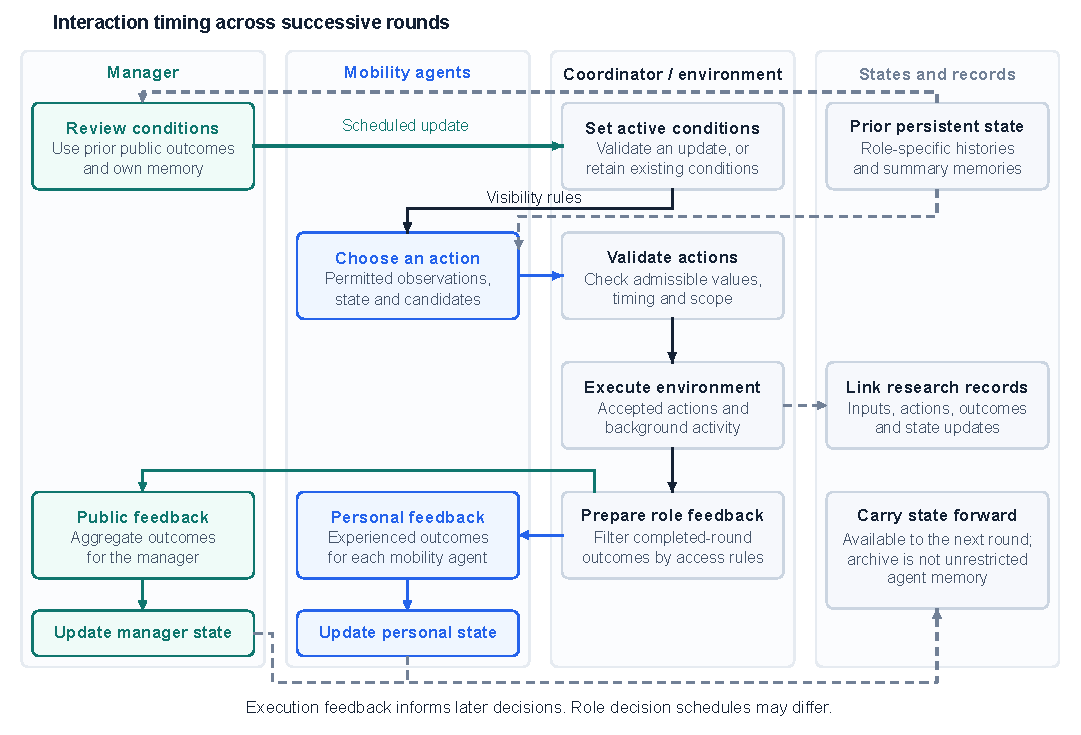
\includegraphics[width=\textwidth, trim=0cm 0cm 0cm 0cm, clip]
        {pic/interaction_timing.pdf}
    \caption{Interaction timing and state updates across
    successive rounds. Solid arrows indicate action and
    feedback flows; dashed arrows indicate state transfer
    or research-record linkage. Execution feedback informs
    subsequent decisions, while the research archive remains
    separate from agent-accessible memory.}
    \label{fig:interaction_timing}
\end{figure}



